% =========================================================================== %

\begin{frame}[t,plain]
\titlepage
\end{frame}

% =========================================================================== %

\begin{frame}{Recap}
%
\begin{columns}[T]
\column{.5\linewidth}
\begin{itemize}
\item Time Complexity
	\begin{itemize}
	\item Measuring directly
	\item Counting Instructions
	\item Big O Notation
	\item Master Theorem
	\end{itemize}
\item Memory Complexity
\item Optimizing for Time Complexity
	\begin{itemize}
	\item Optimize loops
	\item Lazy evaluation
	\item Short Circuits
	\end{itemize}
\end{itemize}
%
\column{.5\linewidth}
\begin{itemize}
\item Writing elegant code
	\begin{itemize}
	\item Plan ahead
	\item Be \emph{fully} aware of what you want to do
	\item Rubber duck method
	\item Bite sized chunks
	\item Sketches and flow diagrams
	\item More time planning than coding
	\item Optimization happes the \emph{second} time you write code
	\item Test each unit
	\end{itemize}
\end{itemize}

\end{columns}
%
\begin{center}
	\emph{Any Questions?}
\end{center}
%
\end{frame}

% =========================================================================== %

\begin{frame}%
%
\begin{columns}[T]
\column{.5\linewidth}
\begin{Large}
	{Ducklings}
\end{Large}
%
\begin{center}
	\vspace{60pt}
	\emph{DUCKLOOP'D?}

	\vspace{6pt}
	Source: \url{https://xkcd.com/537/}
\end{center}
%
\column{.5\linewidth}
\begin{center}
	\includegraphics[width=.38\linewidth]{./gfx/ducklings}\\
\end{center}
\end{columns}

%
\end{frame}

% =========================================================================== %

\begin{frame}[fragile]{Peculiar Behaviour}
%
\begin{tcbraster}[raster columns=2,
                  raster equal height,
                  nobeforeafter,
                  raster column skip=0.5cm]
\begin{codebox}[Example: Generator Objects]
\begin{minted}[fontsize=\scriptsize, linenos]{python3}
gen = (x for x in range(5))

for x in gen :
    print(x)

for x in gen :
    print(x)

rangeObj[0]
\end{minted}
\end{codebox}
%
\begin{cmdbox}[Output: Generator Objects]
\begin{minted}[fontsize=\scriptsize]{text}
0
1
2
3
4

Traceback (most recent call last):
  File "<stdin>", line 1, in <module>
TypeError: 'generator' object is not
  subscriptable

\end{minted}
\end{cmdbox}
\end{tcbraster}
%
\begin{center}
\emph{
	Where is the second \inPy{for}'s output?\\
	What does the Error message mean?
}
\end{center}
%
\end{frame}

% =========================================================================== %

\begin{frame}[fragile]{Generator Objects}
%
\begin{codebox}[Syntax: Generator Objects]
\begin{minted}[fontsize=\scriptsize]{python3}
variable = (expression for variable in iterable)
\end{minted}
\end{codebox}
%
\begin{columns}[T]
\column{.5\linewidth}
\begin{itemize}
\item New syntax: list comprehension with (parentheses)
\item Creates an object that can be looped over
\item Does not pre-compute all elements
\item Instead: Stores rules how to compute the next object
\item And: Last internal state
\end{itemize}
%
\column{.5\linewidth}
\begin{itemize}
\item Results are \enquote{consumed}
\item No automatic restoration
\item Once the last object has been read, the generator is \emph{depleted}
\item No means to skip items or go back
\item[\Thus] No index access (\enquote{not subscriptable})
\end{itemize}
\end{columns}
%
\end{frame}

% =========================================================================== %

\begin{frame}[fragile]{Generator Objects}
%
\begin{columns}[T]
\column{.5\linewidth}
\begin{itemize}
\item New command \inPy{yield}: like \inPy{return}, but:
\item Preserves state of the function left
	\begin{itemize}
	\item All variables remain in memory
	\item Return point is stored
	\end{itemize}
\item When iterating over generator object
	\begin{itemize}
	\item Jump back to where we left it
	\item I.\,e. right after the \inPy{yield} line
	\end{itemize}
\item Again: Can be depleted
\item New instance: \texttt{gen2 = generator()}
\end{itemize}
%
\column{.5\linewidth}
\begin{codebox}[Alternative: Generator Objects]
\begin{minted}[fontsize=\scriptsize, linenos]{python3}
def generator () :
    for x in range(5) :
        yield x

gen = generator()
for x in gen :
    print(x)

for x in gen :
    print(x)
\end{minted}
\end{codebox}
\end{columns}
%
\end{frame}

% =========================================================================== %

\begin{frame}[fragile]
%
\begin{columns}[T]
\column{.5\linewidth}
\begin{Large}
	{Asking Generator Objects for Elements}
	\vspace{6pt}
\end{Large}
\begin{itemize}
\item \inPy{next}: goes through the generator code a single time
\item[\Thus] reads/consumes the \emph{next} value
\item Affects all other constructs reading from the generator
\item[\Thus] \inPy{for} only \enquote{sees} the last three elements
\item \inPy{for} implicitly calls \inPy{next} in each iteration
\end{itemize}
%
\column{.5\linewidth}
\begin{codebox}[Example: \texttt{next}]
\begin{minted}[fontsize=\scriptsize, linenos]{python3}
gen = (x for x in range(5))

print("first :", next(gen))
print("second:", next(gen))

print("the rest:")
for x in gen :
    print(x)
\end{minted}
\end{codebox}
%
\begin{cmdbox}[Output: \texttt{next}]
\begin{minted}[fontsize=\scriptsize]{text}
first : 0
second: 1
the rest:
2
3
4
\end{minted}
\end{cmdbox}
\end{columns}
%
\end{frame}

% =========================================================================== %

\begin{frame}[fragile]{Going Object Oriented}
%
\begin{columns}[T]
\column{.5\linewidth}
\begin{itemize}
\item \inPy{next}: Expects an \emph{iterable}
\item Iterable: Instance of a class with dunder \inPy{__next__}
	\begin{itemize}
	\item Returns the next element in line
	\item Functions with \inPy{yield} automatically generate such an object
	\item May have any internal structure
	\item \inPy{__next__} may affect instance attributes
	\item[\Thus] Evolution of internal state
	\end{itemize}
\end{itemize}
%
\column{.5\linewidth}
\begin{codebox}[Example: \texttt{next}]
\begin{minted}[fontsize=\scriptsize, linenos]{python3}
class Cantina :
  def __next__(self) :
    return "The same song again, okay!"
    
band = Cantina()
print(next(band))
print(next(band))

\end{minted}
\end{codebox}
%
\begin{cmdbox}[Output: \texttt{next}]
\begin{minted}[fontsize=\scriptsize]{text}
The same song again, okay!
The same song again, okay!
\end{minted}
\end{cmdbox}
\end{columns}
%
\end{frame}

% =========================================================================== %

\begin{frame}[fragile]
%
\begin{codebox}[Example: Internal Structure of Automatic Generator Objects]
\begin{minted}[linenos, fontsize=\scriptsize]{python3}
# gen = (x for x in range(5))

class HiddenGeneratorObjectClass :
    def __init__ (self) :
        self.counter = 0
        self.limit   = 5
        self.stride  = 1
    
    def __next__ (self) :
        reVal = self.counter
        self.counter += self.stride
        if self.counter > self.limit :
            raise StopIteration
        else :
            return reVal

gen = HiddenGeneratorObjectClass()

print(next(gen), next(gen), next(gen), next(gen), next(gen))  # 0 1 2 3 4
print(next(gen))                                              # StopIteration
\end{minted}
\end{codebox}
%
\end{frame}

% =========================================================================== %

\begin{frame}[fragile]
%
\begin{warnbox}[Example: Attempting to loop, leftupper=7mm]
\begin{minted}[linenos, fontsize=\scriptsize]{python3}
class HiddenGeneratorObjectClass :
    # ... as before

gen = HiddenGeneratorObjectClass()

for x in gen :
    print(x)
\end{minted}
\end{warnbox}
%
\begin{cmdbox}[Output: Attempting to loop]
\begin{minted}[fontsize=\scriptsize]{text}
  File "/home/blue-chameleon/.config/spyder-py3/temp.py", line 6, in <module>
    for x in gen :

TypeError: 'HiddenGeneratorObjectClass' object is not iterable
\end{minted}
\end{cmdbox}
%
\end{frame}

% =========================================================================== %

\begin{frame}[fragile]{Why This Can't Work}
%
\begin{columns}[T]
\column{.5\linewidth}
\begin{itemize}
\item \emph{Nested} loops over same \texttt{data} source
\item Each loop needs their own counter
\item If a \inPy{list} had a counter, then the inner loop would already consume everything
\item Inner loop would not \enquote{see} the first element in the list
\item Outer loop would not be executed more than once
\item Way out: Helper Object \emph{per loop}
\item Generated by new dunder \inPy{__iter__}
\item If programmed correctly, even allows reusability (hardly ever needed)
\end{itemize}
%
\column{.5\linewidth}
\begin{codebox}[Example: Nested Loops]
\begin{minted}[fontsize=\scriptsize, linenos]{python3}
data = [1, 2]

for x in data :
    print(x)
    for x in data :
        print("  ", x, end="")
    print()
\end{minted}
\end{codebox}
%
\begin{cmdbox}[Output: Nested Loops]
\begin{minted}[fontsize=\scriptsize]{text}
1
   1   2
2
   1   2
\end{minted}
\end{cmdbox}
\end{columns}
%
\end{frame}

% =========================================================================== %

\begin{frame}[fragile]
%
\begin{codebox}[\texttt{for} Loops: Internal mechanics]
\begin{minted}[linenos, fontsize=\scriptsize]{python3}
# for x in container :
#     statements

iterObj = iter(container)
while True :
    try :
        x = next(iterObj)
    except StopIteration as e :
        break
    
    statements
\end{minted}
\end{codebox}
%
As you can imagine, \inPy{iter} calls \inPy{__iter__}.
%
\end{frame}

% =========================================================================== %

\begin{frame}[fragile]
%
\begin{codebox}[Example: Complete Iterable Class]
\begin{minted}[linenos, fontsize=\scriptsize]{python3}
class HiddenGeneratorObjectClass :
    def __init__ (self) :
        self.counter = 0
        self.limit   = 5
        self.stride  = 1
    
    def __next__ (self) :
        reVal = self.counter
        self.counter += self.stride
        if self.counter > self.limit :
            raise StopIteration
        else :
            return reVal

    def __iter__ (self) :             # in more complex scenarios, this will return
        return self                   # an instance of a different helper class.

gen = HiddenGeneratorObjectClass()
for x in gen :
    print(x)
\end{minted}
\end{codebox}
%
\end{frame}

% =========================================================================== %

\begin{frame}[fragile]{Put It to Use: Linked Lists}
%
\begin{itemize}
\item Consider an array:\\
	\texttt{[1, 2, 3, 4, 5]}
\item Insert \texttt{0} at the start of the array
\item Requires moving \emph{all} objects by one spot to the right
\item[\Thus] Runtime: $\mathcal{O}(N)$
\end{itemize}
%
\begin{tcolorbox}[title=Visualization: Inserting into an Array]
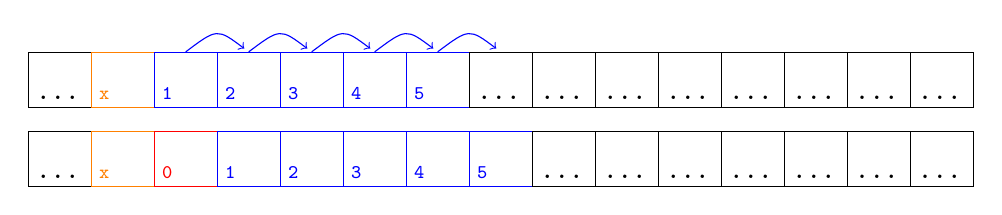
\begin{tikzpicture}
  [ 
    cell/.style={text width=6mm,
    text height=5mm, draw=black, inner sep=1mm},
    ld/.style={draw=blue,shorten >=2pt,->}
  ]
  \node (c01) at ( 0.0,0) [cell]       {\ttfamily \ldots};
  \node (c02) at ( 0.8,0) [cell, orange] {\ttfamily \scriptsize x};
  \node (c03) at ( 1.6,0) [cell, blue] {\ttfamily \scriptsize 1};
  \node (c04) at ( 2.4,0) [cell, blue] {\ttfamily \scriptsize 2};
  \node (c05) at ( 3.2,0) [cell, blue] {\ttfamily \scriptsize 3};
  \node (c06) at ( 4.0,0) [cell, blue] {\ttfamily \scriptsize 4};
  \node (c07) at ( 4.8,0) [cell, blue] {\ttfamily \scriptsize 5};
  \node (c08) at ( 5.6,0) [cell]       {\ttfamily \ldots};
  \node (c09) at ( 6.4,0) [cell]       {\ttfamily \ldots};
  \node (c10) at ( 7.2,0) [cell]       {\ttfamily \ldots};
  \node (c11) at ( 8.0,0) [cell]       {\ttfamily \ldots};
  \node (c12) at ( 8.8,0) [cell]       {\ttfamily \ldots};
  \node (c13) at ( 9.6,0) [cell]       {\ttfamily \ldots};
  \node (c14) at (10.4,0) [cell]       {\ttfamily \ldots};
  \node (c15) at (11.2,0) [cell]       {\ttfamily \ldots};
  
  \draw [ld] (c03.north) .. controls +(0.4,0.3) .. (c04.north);
  \draw [ld] (c04.north) .. controls +(0.4,0.3) .. (c05.north);
  \draw [ld] (c05.north) .. controls +(0.4,0.3) .. (c06.north);
  \draw [ld] (c06.north) .. controls +(0.4,0.3) .. (c07.north);
  \draw [ld] (c07.north) .. controls +(0.4,0.3) .. (c08.north);
  
  \node (c01) at ( 0.0, -1) [cell]       {\ttfamily \ldots};
  \node (c02) at ( 0.8, -1) [cell, orange] {\ttfamily \scriptsize x};
  \node (c03) at ( 1.6, -1) [cell, red ] {\ttfamily \scriptsize 0};
  \node (c04) at ( 2.4, -1) [cell, blue] {\ttfamily \scriptsize 1};
  \node (c05) at ( 3.2, -1) [cell, blue] {\ttfamily \scriptsize 2};
  \node (c06) at ( 4.0, -1) [cell, blue] {\ttfamily \scriptsize 3};
  \node (c07) at ( 4.8, -1) [cell, blue] {\ttfamily \scriptsize 4};
  \node (c08) at ( 5.6, -1) [cell, blue] {\ttfamily \scriptsize 5};
  \node (c09) at ( 6.4, -1) [cell]       {\ttfamily \ldots};
  \node (c10) at ( 7.2, -1) [cell]       {\ttfamily \ldots};
  \node (c11) at ( 8.0, -1) [cell]       {\ttfamily \ldots};
  \node (c12) at ( 8.8, -1) [cell]       {\ttfamily \ldots};
  \node (c13) at ( 9.6, -1) [cell]       {\ttfamily \ldots};
  \node (c14) at (10.4, -1) [cell]       {\ttfamily \ldots};
  \node (c15) at (11.2, -1) [cell]       {\ttfamily \ldots};
\end{tikzpicture}
\end{tcolorbox}
%
\end{frame}

% =========================================================================== %

\begin{frame}[fragile]{Linked Lists -- Structure and Use Case}
%
\begin{itemize}
\item Common Requirement
	\begin{itemize}
	\item Stack or FIFO structure (first in, first out)
	\item Fast at adding/removing
	\item Random access (\ie indexed acces) to elements needs not be fast\\
		(always access first element)
	\end{itemize}
\item Realization
	\begin{itemize}
	\item List elements are \enquote{anywhere} in memory, \ie not in sequence
	\item Each element \enquote{knows} where its successor is located
	\item Helper \inPy{class ListElement}, comprising of \texttt{realData} and \texttt{nextNode}
	\item Commonly also: \inPy{class LinkedList}
		\begin{itemize}
		\item Knows entry point
		\item Keeps track of runtime variables
		\item Offers convenience methods
		\end{itemize}
	\end{itemize}
\end{itemize}
%
\end{frame}

% =========================================================================== %

\begin{frame}[fragile]
%
\begin{codebox}[Linked List Element Instances]
\begin{minted}[linenos, fontsize=\scriptsize]{python3}
class ListElement
    def __init__(self, realData, nextNode = None) :
        self.realData = realData
        self.nextNode = nextNode
\end{minted}
\end{codebox}
%
\begin{tcolorbox}[title=Visualization: Linked List]
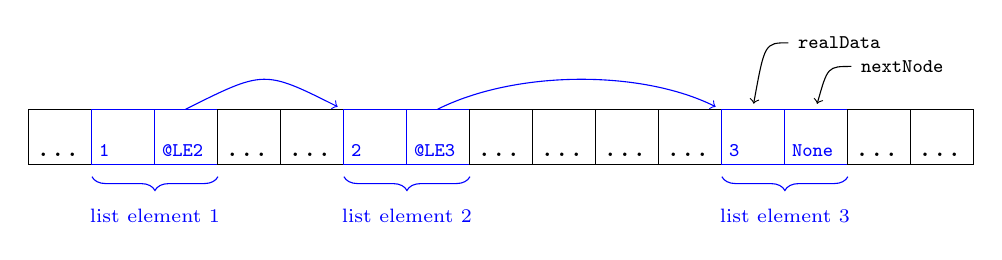
\begin{tikzpicture}
  [ 
    cell/.style={text width=6mm,
    text height=5mm, draw=black, inner sep=1mm},
    ld/.style={draw=blue,shorten >=2pt,->}
  ]
  \node (c01) at ( 0.0,0) [cell]       {\ttfamily \ldots};
  \node (c02) at ( 0.8,0) [cell, blue] {\ttfamily \scriptsize 1};
  \node (c03) at ( 1.6,0) [cell, blue] {\ttfamily \scriptsize @LE2};
  \node (c04) at ( 2.4,0) [cell]       {\ttfamily \ldots};
  \node (c05) at ( 3.2,0) [cell]       {\ttfamily \ldots};
  \node (c06) at ( 4.0,0) [cell, blue] {\ttfamily \scriptsize 2};
  \node (c07) at ( 4.8,0) [cell, blue] {\ttfamily \scriptsize @LE3};
  \node (c08) at ( 5.6,0) [cell]       {\ttfamily \ldots};
  \node (c09) at ( 6.4,0) [cell]       {\ttfamily \ldots};
  \node (c10) at ( 7.2,0) [cell]       {\ttfamily \ldots};
  \node (c11) at ( 8.0,0) [cell]       {\ttfamily \ldots};
  \node (c12) at ( 8.8,0) [cell, blue] {\ttfamily \scriptsize 3};
  \node (c13) at ( 9.6,0) [cell, blue] {\ttfamily \scriptsize None};
  \node (c14) at (10.4,0) [cell]       {\ttfamily \ldots};
  \node (c15) at (11.2,0) [cell]       {\ttfamily \ldots};
  
  \draw [ld] (c03.north) .. controls +(1.0,0.5) and +(-1.0, 0.5) .. (c06.north west);
  \draw [ld] (c07.north) .. controls +(1.0,0.5) and +(-1.0, 0.5) .. (c12.north west);
  
  \node (x1) at ( 9.9, 1.2) {\ttfamily \scriptsize  realData};
  \node (x2) at (10.7, 0.9) {\ttfamily \scriptsize nextNode};
  
  \draw [ld, black] (x1.west) .. controls +(-0.3,0.0) .. (c12.north);
  \draw [ld, black] (x2.west) .. controls +(-0.3,0.0) .. (c13.north);
  
  \draw [decorate, decoration={brace, amplitude=5pt, mirror}, xshift=-4pt, yshift=0pt, blue]
  		(0.55, -0.5) -- (2.15, -0.5) 
  		node [midway, yshift=-0.5cm]
		(I1) {\scriptsize list element 1};
  \draw [decorate, decoration={brace, amplitude=5pt, mirror}, xshift=-4pt, yshift=0pt, blue]
  		(3.75, -0.5) -- (5.35, -0.5) 
  		node [midway, yshift=-0.5cm]
		(I2) {\scriptsize list element 2};
  \draw [decorate, decoration={brace, amplitude=5pt, mirror}, xshift=-4pt, yshift=0pt, blue]
  		(8.55, -0.5) -- (10.15, -0.5) 
  		node [midway, yshift=-0.5cm]
		(I3) {\scriptsize list element 3};
\end{tikzpicture}

\vspace{6pt}
The attribute \texttt{nextNode} of the \emph{last} element is always \inPy{None}.
\end{tcolorbox}
%
\end{frame}

% =========================================================================== %

\begin{frame}[fragile]
%
\begin{tcolorbox}[title=Visualization: Insertion in the Middle of a Linked List]
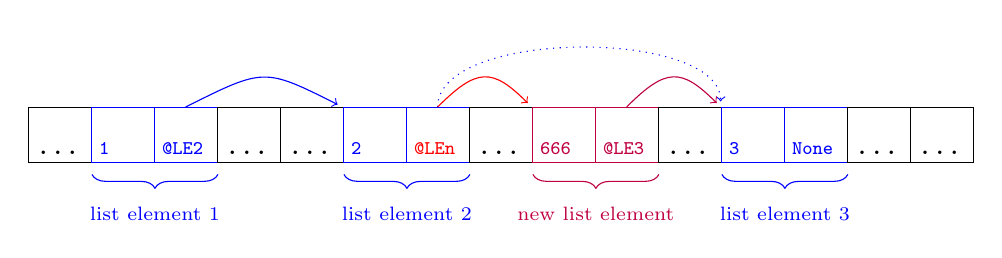
\begin{tikzpicture}
  [ 
    cell/.style={text width=6mm,
    text height=5mm, draw=black, inner sep=1mm},
    ld/.style={draw=blue,shorten >=2pt,->}
  ]
  \node (c01) at ( 0.0,0) [cell]         {\ttfamily \ldots};
  \node (c02) at ( 0.8,0) [cell, blue]   {\ttfamily \scriptsize 1};
  \node (c03) at ( 1.6,0) [cell, blue]   {\ttfamily \scriptsize @LE2};
  \node (c04) at ( 2.4,0) [cell]         {\ttfamily \ldots};
  \node (c05) at ( 3.2,0) [cell]         {\ttfamily \ldots};
  \node (c06) at ( 4.0,0) [cell, blue]   {\ttfamily \scriptsize 2};
  \node (c07) at ( 4.8,0) [cell, blue]   {\ttfamily \scriptsize \textcolor{red}{@LEn}};
  \node (c08) at ( 5.6,0) [cell]         {\ttfamily \ldots};
  \node (c09) at ( 6.4,0) [cell, purple] {\ttfamily \scriptsize 666};
  \node (c10) at ( 7.2,0) [cell, purple] {\ttfamily \scriptsize @LE3};
  \node (c11) at ( 8.0,0) [cell]         {\ttfamily \ldots};
  \node (c12) at ( 8.8,0) [cell, blue]   {\ttfamily \scriptsize 3};
  \node (c13) at ( 9.6,0) [cell, blue]   {\ttfamily \scriptsize None};
  \node (c14) at (10.4,0) [cell]         {\ttfamily \ldots};
  \node (c15) at (11.2,0) [cell]         {\ttfamily \ldots};
  
  \draw [ld]         (c03.north) .. controls +(1.0,0.5) and +(-1.0, 0.5) .. (c06.north west);
  \draw [ld, dotted] (c07.north) .. controls +(0.0,1.0) and +(-0.0, 1.0) .. (c12.north west);
  \draw [ld, red]    (c07.north) .. controls +(0.5,0.5) and +(-0.5, 0.5) .. (c09.north west);
  \draw [ld, purple] (c10.north) .. controls +(0.5,0.5) and +(-0.5, 0.5) .. (c12.north west);

  \draw [decorate, decoration={brace, amplitude=5pt, mirror}, xshift=-4pt, yshift=0pt, blue]
  		(0.55, -0.5) -- (2.15, -0.5) 
  		node [midway, yshift=-0.5cm]
		(I1) {\scriptsize list element 1};
  \draw [decorate, decoration={brace, amplitude=5pt, mirror}, xshift=-4pt, yshift=0pt, blue]
  		(3.75, -0.5) -- (5.35, -0.5) 
  		node [midway, yshift=-0.5cm]
		(I2) {\scriptsize list element 2};
  \draw [decorate, decoration={brace, amplitude=5pt, mirror}, xshift=-4pt, yshift=0pt, blue]
  		(8.55, -0.5) -- (10.15, -0.5) 
  		node [midway, yshift=-0.5cm]
		(I3) {\scriptsize list element 3};
  \draw [decorate, decoration={brace, amplitude=5pt, mirror}, xshift=-4pt, yshift=0pt, purple]
  		(6.15, -0.5) -- (7.75, -0.5) 
  		node [midway, yshift=-0.5cm]
		(I4) {\scriptsize new list element};
\end{tikzpicture}
%
\begin{itemize}
\item Prepare new element
\item \texttt{nextNode} refers to successor
\item update \texttt{nextNode} in predecessor
\end{itemize}
\end{tcolorbox}
%
\end{frame}

% =========================================================================== %

\begin{frame}[fragile]
%
\begin{tcolorbox}[title=Visualization: Insertion at the End of a Linked List]
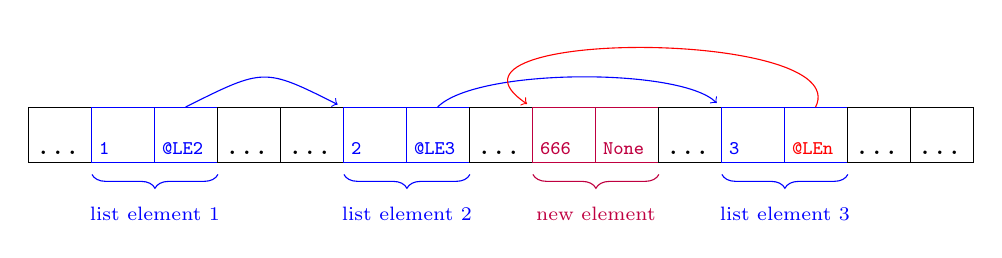
\begin{tikzpicture}
  [ 
    cell/.style={text width=6mm,
    text height=5mm, draw=black, inner sep=1mm},
    ld/.style={draw=blue,shorten >=2pt,->}
  ]
  \node (c01) at ( 0.0,0) [cell]         {\ttfamily \ldots};
  \node (c02) at ( 0.8,0) [cell, blue]   {\ttfamily \scriptsize 1};
  \node (c03) at ( 1.6,0) [cell, blue]   {\ttfamily \scriptsize @LE2};
  \node (c04) at ( 2.4,0) [cell]         {\ttfamily \ldots};
  \node (c05) at ( 3.2,0) [cell]         {\ttfamily \ldots};
  \node (c06) at ( 4.0,0) [cell, blue]   {\ttfamily \scriptsize 2};
  \node (c07) at ( 4.8,0) [cell, blue]   {\ttfamily \scriptsize @LE3};
  \node (c08) at ( 5.6,0) [cell]         {\ttfamily \ldots};
  \node (c09) at ( 6.4,0) [cell, purple] {\ttfamily \scriptsize 666};
  \node (c10) at ( 7.2,0) [cell, purple] {\ttfamily \scriptsize None};
  \node (c11) at ( 8.0,0) [cell]         {\ttfamily \ldots};
  \node (c12) at ( 8.8,0) [cell, blue]   {\ttfamily \scriptsize 3};
  \node (c13) at ( 9.6,0) [cell, blue]   {\ttfamily \scriptsize \textcolor{red}{@LEn}};
  \node (c14) at (10.4,0) [cell]         {\ttfamily \ldots};
  \node (c15) at (11.2,0) [cell]         {\ttfamily \ldots};
  
  \draw [ld]         (c03.north) .. controls +(1.0,0.5) and +(-1.0, 0.5) .. (c06.north west);
  \draw [ld]         (c07.north) .. controls +(0.5,0.5) and +(-0.5, 0.5) .. (c12.north west);
  \draw [ld, red]    (c13.north) .. controls +(0.5,1.0) and +(-1.5, 1.0) .. (c09.north west);

  \draw [decorate, decoration={brace, amplitude=5pt, mirror}, xshift=-4pt, yshift=0pt, blue]
  		(0.55, -0.5) -- (2.15, -0.5) 
  		node [midway, yshift=-0.5cm]
		(I1) {\scriptsize list element 1};
  \draw [decorate, decoration={brace, amplitude=5pt, mirror}, xshift=-4pt, yshift=0pt, blue]
  		(3.75, -0.5) -- (5.35, -0.5) 
  		node [midway, yshift=-0.5cm]
		(I2) {\scriptsize list element 2};
  \draw [decorate, decoration={brace, amplitude=5pt, mirror}, xshift=-4pt, yshift=0pt, blue]
  		(8.55, -0.5) -- (10.15, -0.5) 
  		node [midway, yshift=-0.5cm]
		(I3) {\scriptsize list element 3};
  \draw [decorate, decoration={brace, amplitude=5pt, mirror}, xshift=-4pt, yshift=0pt, purple]
  		(6.15, -0.5) -- (7.75, -0.5) 
  		node [midway, yshift=-0.5cm]
		(I4) {\scriptsize new element};
\end{tikzpicture}
%
\begin{itemize}
\item Prepare new list element
\item \texttt{nextNode} is \texttt{None}
\item Update \texttt{nextNode} in previously last list element
\end{itemize}
\end{tcolorbox}
%
\end{frame}

% =========================================================================== %

\begin{frame}
%
\begin{tcolorbox}[title=Visualization: Insertion at the Front of a Linked List]
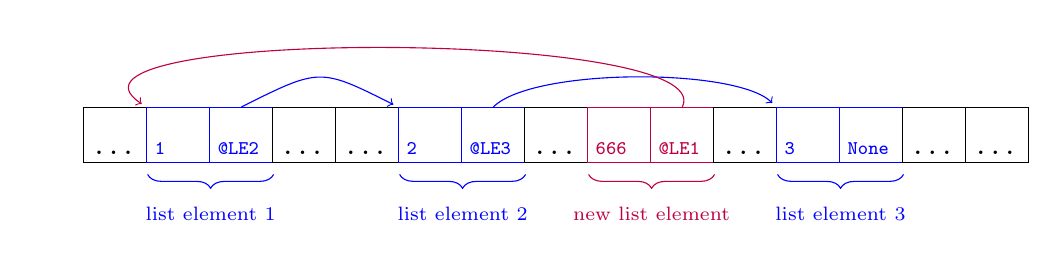
\begin{tikzpicture}
  [ 
    cell/.style={text width=6mm,
    text height=5mm, draw=black, inner sep=1mm},
    ld/.style={draw=blue,shorten >=2pt,->}
  ]
  \node (c01) at ( 0.0,0) [cell]         {\ttfamily \ldots};
  \node (c02) at ( 0.8,0) [cell, blue]   {\ttfamily \scriptsize 1};
  \node (c03) at ( 1.6,0) [cell, blue]   {\ttfamily \scriptsize @LE2};
  \node (c04) at ( 2.4,0) [cell]         {\ttfamily \ldots};
  \node (c05) at ( 3.2,0) [cell]         {\ttfamily \ldots};
  \node (c06) at ( 4.0,0) [cell, blue]   {\ttfamily \scriptsize 2};
  \node (c07) at ( 4.8,0) [cell, blue]   {\ttfamily \scriptsize @LE3};
  \node (c08) at ( 5.6,0) [cell]         {\ttfamily \ldots};
  \node (c09) at ( 6.4,0) [cell, purple] {\ttfamily \scriptsize 666};
  \node (c10) at ( 7.2,0) [cell, purple] {\ttfamily \scriptsize @LE1};
  \node (c11) at ( 8.0,0) [cell]         {\ttfamily \ldots};
  \node (c12) at ( 8.8,0) [cell, blue]   {\ttfamily \scriptsize 3};
  \node (c13) at ( 9.6,0) [cell, blue]   {\ttfamily \scriptsize None};
  \node (c14) at (10.4,0) [cell]         {\ttfamily \ldots};
  \node (c15) at (11.2,0) [cell]         {\ttfamily \ldots};
  
  \draw [ld]         (c03.north) .. controls +(1.0,0.5) and +(-1.0, 0.5) .. (c06.north west);
  \draw [ld]         (c07.north) .. controls +(0.5,0.5) and +(-0.5, 0.5) .. (c12.north west);
  \draw [ld, purple] (c10.north) .. controls +(0.5,1.0) and +(-1.5, 1.0) .. (c02.north west);

  \draw [decorate, decoration={brace, amplitude=5pt, mirror}, xshift=-4pt, yshift=0pt, blue]
  		(0.55, -0.5) -- (2.15, -0.5) 
  		node [midway, yshift=-0.5cm]
		(I1) {\scriptsize list element 1};
  \draw [decorate, decoration={brace, amplitude=5pt, mirror}, xshift=-4pt, yshift=0pt, blue]
  		(3.75, -0.5) -- (5.35, -0.5) 
  		node [midway, yshift=-0.5cm]
		(I2) {\scriptsize list element 2};
  \draw [decorate, decoration={brace, amplitude=5pt, mirror}, xshift=-4pt, yshift=0pt, blue]
  		(8.55, -0.5) -- (10.15, -0.5) 
  		node [midway, yshift=-0.5cm]
		(I3) {\scriptsize list element 3};
  \draw [decorate, decoration={brace, amplitude=5pt, mirror}, xshift=-4pt, yshift=0pt, purple]
  		(6.15, -0.5) -- (7.75, -0.5) 
  		node [midway, yshift=-0.5cm]
		(I4) {\scriptsize new list element};
\end{tikzpicture}
%
\begin{itemize}
\item Only prepare new element!
\item Entry Point has changed
\item[\Thus] \inPy{clas ListRoot}
\end{itemize}
\end{tcolorbox}
%
\end{frame}

% =========================================================================== %

\begin{frame}
%
\begin{tcolorbox}[title=Visualization: Deleting from a Linked List]
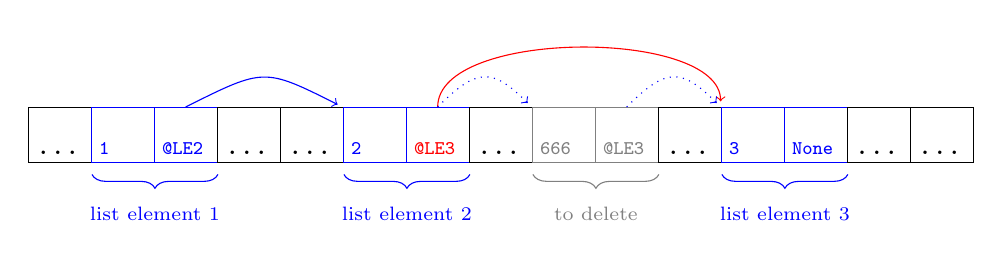
\begin{tikzpicture}
  [ 
    cell/.style={text width=6mm,
    text height=5mm, draw=black, inner sep=1mm},
    ld/.style={draw=blue,shorten >=2pt,->}
  ]

  \node (c01) at ( 0.0,0) [cell]         {\ttfamily \ldots};
  \node (c02) at ( 0.8,0) [cell, blue]   {\ttfamily \scriptsize 1};
  \node (c03) at ( 1.6,0) [cell, blue]   {\ttfamily \scriptsize @LE2};
  \node (c04) at ( 2.4,0) [cell]         {\ttfamily \ldots};
  \node (c05) at ( 3.2,0) [cell]         {\ttfamily \ldots};
  \node (c06) at ( 4.0,0) [cell, blue]   {\ttfamily \scriptsize 2};
  \node (c07) at ( 4.8,0) [cell, blue]   {\ttfamily \scriptsize \textcolor{red}{@LE3}};
  \node (c08) at ( 5.6,0) [cell]         {\ttfamily \ldots};
  \node (c09) at ( 6.4,0) [cell, gray]   {\ttfamily \scriptsize 666};
  \node (c10) at ( 7.2,0) [cell, gray]   {\ttfamily \scriptsize @LE3};
  \node (c11) at ( 8.0,0) [cell]         {\ttfamily \ldots};
  \node (c12) at ( 8.8,0) [cell, blue]   {\ttfamily \scriptsize 3};
  \node (c13) at ( 9.6,0) [cell, blue]   {\ttfamily \scriptsize None};
  \node (c14) at (10.4,0) [cell]         {\ttfamily \ldots};
  \node (c15) at (11.2,0) [cell]         {\ttfamily \ldots};
  
  \draw [ld]         (c03.north) .. controls +(1.0,0.5) and +(-1.0, 0.5) .. (c06.north west);
  \draw [ld, red]    (c07.north) .. controls +(0.0,1.0) and +(-0.0, 1.0) .. (c12.north west);
  \draw [ld, dotted] (c07.north) .. controls +(0.5,0.5) and +(-0.5, 0.5) .. (c09.north west);
  \draw [ld, dotted] (c10.north) .. controls +(0.5,0.5) and +(-0.5, 0.5) .. (c12.north west);

  \draw [decorate, decoration={brace, amplitude=5pt, mirror}, xshift=-4pt, yshift=0pt, blue]
  		(0.55, -0.5) -- (2.15, -0.5) 
  		node [midway, yshift=-0.5cm]
		(I1) {\scriptsize list element 1};
  \draw [decorate, decoration={brace, amplitude=5pt, mirror}, xshift=-4pt, yshift=0pt, blue]
  		(3.75, -0.5) -- (5.35, -0.5) 
  		node [midway, yshift=-0.5cm]
		(I2) {\scriptsize list element 2};
  \draw [decorate, decoration={brace, amplitude=5pt, mirror}, xshift=-4pt, yshift=0pt, blue]
  		(8.55, -0.5) -- (10.15, -0.5) 
  		node [midway, yshift=-0.5cm]
		(I3) {\scriptsize list element 3};
  \draw [decorate, decoration={brace, amplitude=5pt, mirror}, xshift=-4pt, yshift=0pt, gray]
  		(6.15, -0.5) -- (7.75, -0.5) 
  		node [midway, yshift=-0.5cm]
		(I4) {\scriptsize to delete};
\end{tikzpicture}
%
\begin{itemize}
\item Update \texttt{nextNode} in predecessor or update entry point:\\
	\texttt{nextNode} of \texttt{toDelete}
\item That's all!
\end{itemize}
\end{tcolorbox}
%
\end{frame}

% =========================================================================== %\\

\begin{frame}
%
\begin{hintbox}[Limited Implementation]
We've discussed inserting in the middle and at the end for the sake of completeness. However, most of the time only \texttt{push} and \texttt{pop} (insert/delete from the front) are implemented. This is because inserting/deleting at/from arbitrary points requires finding these points, which can takes $\mathcal{O}(N)$ FLOPs, thereby eliminating the advantage of the linked list. Only at the front of the list, this paper chase is not necessary and we can take full advantage of the list.

In the example below, we find \texttt{push}, \texttt{pop} as well as random read/write access, but no generic insert/remove method for that very reason.
\end{hintbox}
%
\end{frame}

% =========================================================================== %

\begin{frame}[fragile]{Implementation}
%
\begin{center}
\begin{Large}
	File \texttt{001-linkedList-a.py}
\end{Large}
\end{center}
%
\end{frame}


% =========================================================================== %

\begin{frame}[fragile]{Making it Compatible with \inPy{for}}
%
\begin{itemize}
\item Introduce new \inPy{class LinkedListIterable}
\item Knows next in line (instance attribute)
\item Has dunder \inPy{__next__}
	\begin{itemize}
	\item returns and updates next in line
	\item raises \inPy{StopIteration} when done
	\end{itemize}
\item Is returned by \inPy{__iter__} from \inPy{class LinkedList}
\end{itemize}
%
\end{frame}

% =========================================================================== %

\begin{frame}[fragile]
%
\begin{codebox}[Iterable Linked List]
\begin{minted}[linenos, fontsize=\scriptsize]{python3}
class LinkedListIterable :
    def __init__ (self, current) :
        self.current = current
    def __next__ (self) :
        if self.current :
            reVal = self.current.realData
            self.current = self.current.nextNode
            return reVal
        else :
            raise StopIteration()

class LinkedList :
    # as before ...
    def __iter__ (self) :
        return LinkedListIterable(self.first)

myList = LinkedList()
# append data...

for line in myList :
    print(line)
\end{minted}
\end{codebox}
%
\end{frame}

% =========================================================================== %\\

\begin{frame}
%
\begin{hintbox}[There's More!]
Based on the ideas of a linked list, there are similar structures, such as
\begin{itemize}
\item Doubly linked list (each \texttt{ListElement} knows \texttt{nextNode} \emph{and} \texttt{prevNode})\\
	\Thus\; LIFO (\emph{last} in, first out), traversible in both directions
\item Trees (the \texttt{nextNode} entry is a list of elements hierarchically lower than the self, which can have child elements themselves)
\item Binary search tree (a tree structure with built-in sorting)
\item Red-Black-Trees (a more sophisticated binary search tree with self-regulating properties)
\item ...
\end{itemize}

Do follow the course \emph{Algorithmen und Datenstrukturen} (each summer term, Dr. Stefan Solbrig) if you want to see more.
\end{hintbox}
%
\end{frame}